\documentclass{IEEEtran}

\usepackage[utf8]{inputenc} % set input encoding (not needed with XeLaTeX)
%\usepackage{geometry}
%\geometry{letterpaper}
%%% Examples of Article customizations
% These packages are optional, depending whether you want the features they provide.
% See the LaTeX Companion or other references for full information.



\usepackage{graphicx} % support the \includegraphics command and options

% \usepackage[parfill]{parskip} % Activate to begin paragraphs with an empty line rather than an indent

%%% PACKAGES
\usepackage{url}
\usepackage{booktabs} % for much better looking tables
\usepackage{array} % for better arrays (eg matrices) in maths
\usepackage{paralist} % very flexible & customisable lists (eg. enumerate/itemize, etc.)
\usepackage{verbatim} % adds environment for commenting out blocks of text & for better verbatim
\usepackage{subfig} % make it possible to include more than one captioned figure/table in a single float
\usepackage{algorithm} 
\usepackage{algorithmic}
\usepackage{amsmath}



% These packages are all incorporated in the memoir class to one degree or another...

%%% HEADERS & FOOTERS
%\usepackage{fancyhdr} % This should be set AFTER setting up the page geometry
%\pagestyle{fancy} % options: empty , plain , fancy
%\renewcommand{\headrulewidth}{0pt} % customise the layout...
%\lhead{}\chead{}\rhead{}
%\lfoot{}\cfoot{\thepage}\rfoot{}

%%% END Article customizations

%%% The "real" document content comes below...

\title{VHash: An Optimized Voronoi-Based Distributed Hash Table }
\author{Double Blind}
%\author{Brendan Benshoof \qquad Andrew Rosen  \\Department of Computer Science, Georgia State University\\  bbenshoof@cs.gsu.edu \qquad rosen@cs.gsu.edu }
\date{} % Activate to display a given date or no date (if empty),
         % otherwise the current date is printed 

\begin{document}
\maketitle

\begin{abstract}
%1. State the problem
Distributed Hash Tables (DHT) provide a fast and robust decentralized means of key-value storage and retrieval and are typically used in Peer-to-Peer applications.
DHTs assign nodes a single identifier derived from the hash of their IP address and port, which results in a random overlay network.   
%2. Say why it’s an interesting problem
A random overlay network is not explicitly optimized for certain metrics, such as latency, trust, energy, or hops on an overlay network.  It is often desirable to generate an overlay network that is optimized for one or more specific metrics.

%3. Say what your solution achieves
This paper presents VHash, a DHT protocol to construct an overlay optimized for such metrics. 
VHash exploits a fast and efficient Delaunay Triangulation heuristic in a geometric space. 
%4. Say what follows from your solution
We used VHash to generate an overlay with edges that minimize latency. 
While we focused on latency in this paper, VHash optimizes on any defined metrics.
This overlay outperformed an overlay generated by the Chord DHT protocol in terms of lookup time.
VHash provides a robust, scalable, and efficient distributed lookup service.

\end{abstract}
%  We could use a different config 
% networks are only hpped
% we can do non-euclidean metrics if we have a non-euclidean distance and midpoint definition

\section{Introduction}
A Distributed Hash Table is used provide an overlay network for many P2P applications. %State of the art DHT techniques are built on trees or ring structures to ensure that the routing distance is $O(lg(n))$ hops between nodes. 
%keep?
%In the vast majority of Distributed Hash Tables, such as Chord \cite{chord}, Kademlia\cite{kademlia}, Pastry \cite{pastry}, a node is mapped key on a 1-dimensional keyspace.  This key is chosen via a hash function, such as SHA-1, ensuring that nodes are randomly and uniformly the overlay network.
%keep?
%This provides the network with load balancing properties.  Since files are assigned keys in a similar manner to nodes, the node are distributed evenly ac.  The distribution also provides fault tolerance;  if all the nodes located in a real geographic region were suddenly taken offline, the damage to the network would be spread uniformly throughout the network and maintenance would repair the damage.%
Each node in the overlay network maintains a routing table of a subset of other nodes in the overlay.  
The configuration and rules of the routing table vary from one protocol to another.
In a DHT the entries of the routing tables may be separated by powers of 2 \cite{chord}, be determined by shared prefixes \cite{pastry}, or be chosen according to a probabilistic distribution \cite{kleinberg2000navigation}, but the goal is to minimize the number of overlay hops the distributed lookup needs to make. 


%The ``problem''
%This is the correct choice make if there is no other information to act on during lookup or routing. 
A routing table created to minimize overlay hops does not necessarily create routes with minimized latency.
What if more information about the nodes could be encoded as part of the overlay, such as the node's latency?
Problems like latency require embedding a graph into coordinates in the metric space such as to minimize errors in inter-node distance.
If each node is defined as object in this space we can then use a distance function to choose the shortest path over these metrics and approximate a desired behavior, in this case minimum latency.


This opens up two problems:
How to we create and maintain a DHT based on an arbitrary metric space?
How do we usefully embed inter-node latency and other important routing information into that metric space's coordinate system?

VHash is a DHT designed to take inter-node latency information into account when generating an overlay.
Other network metrics could easily be applied to VHash.
VHash creates an approximation of a Voronoi network and Delaunay Triangulation to define the routing tables and dictate where content is stored in the network.
We accomplish this by assigning each node $d$ coordinates, rather than than a single key.
We use a basic spring model to embed inter-node latency graph in the overlay.
A result of this is that nodes in VHash  can \emph{move} through the metric space over the lifetime of the node;  their position is not necessarily fixed.
Our paper presents the following:

\begin{itemize}
	\item We describe the VHash protocol (Section II) and the underlying approximation algorithm of overlay's Delaunay Trinangulation and the corresponding Voronoi diagrams.
    Our approximation is distributed, greedy, efficient, and accurate in arbitrary number of dimensions and creates an overlay with edges that minimize distance over network metrics while maintaining robustness, scalability, and polylogarithmic lookup time in overlay hops.
	\item We use VHash to provide us with an overlay for embedding network metrics.
    We present our basic spring model for embedding nodes in the overlay with latency information and discuss other network metrics that can be used with VHash (Section III).
	\item We created simulations (Section IV) to prove that the overlays created by VHash are accurate enough for routing messages from arbitrary source nodes to random destination locations.
    We also show that by embedding the latency graph, our routing dramatically outperforms Chord (and by extension, other overlays with $\lg(n)$-sized routing tables) in terms of latency.
	\item We compare the VHash protocol to the other protocols that are based off of Voronoi region approximation (Section V).
	\item We discuss future work that follows from our what plans we have for embedding different problems using VHash (Section VI).
\end{itemize}


\section{VHash}
Nodes in the VHash network periodically gossip with other nodes, exchanging information about theirs peers and use the approximation algorithm to refine its list of neighbors.
These neighbors approximate the node's Voronoi region and it's corresponding responsibilities.
This approximation algorithm is fast and can be used for spaces with an arbitrary number of dimensions.

\subsection{Voronoi Regions in DHTs}
A Voronoi diagram is the division of a space into cells or regions along a set of objects $O$ such that all the points in a particular region are closer to one object than any other object.  
We refer to the region owned by an object as that object's Voronoi region.
The Delaunay Triangulation of this same space along the same set of objects is defined by the edges such that no object is inside the circumcircle of any triangle formed by the edges \cite{geoalg}.  
The Voronoi diagram and Delaunay Triangulation are dual problems, as an edge between two objects in a Delaunay Triangulation exists if and only if those object's Voronoi region border each other.  
This means that solving either problem will yield the solution to both.   An example Voronoi diagram is shown in Figure \ref{voro-ex}


\begin{figure}
	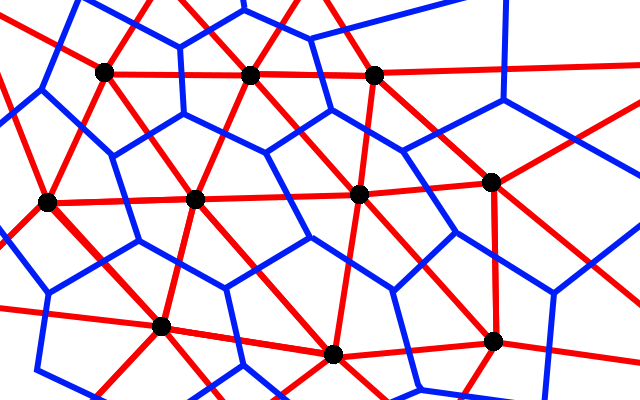
\includegraphics[width=\linewidth]{voronoi-example}
	\caption{An example Voronoi diagram for objects on a 2-dimensional toroidal space.  The black lines correspond to the edges of the Delaunay Triangulation}
	\label{voro-ex}
\end{figure}

In our network, the nodes are the objects of the Voronoi diagram and their regions define the regions they are responsible for.  The edges created by the Deluanay Triangulation correspond to the connections between neighboring nodes.  Computing Voronoi diagrams in a distributed and generalized fashion is prohibitively time expensive.
A greedy approximation of the Voronoi regions is sufficient for the VHash protocol.
We created a new greedy, online algorithm that approximates and maintains the set of peers defining the node's Voronoi region and Delaunay Triangulation.




A formal and thorough description of Voronoi diagrams as well as their applications can be found in \cite{aurenhammer1991voronoi}.

Arguably all DHTs are built on the concept of Vornoi regions.
In all DHT's currently a node is responsible for all points in it's hash space to which it is the ``closest'' node.
These DHTs have carefully chosen metric spaces such that these regions are very simple to calculate.
For example Chord and similar ring based DHTs utilize a unidirectional one dimensional ring as their metric space, such that the region for which a node is responsible is the region between it and it's predecessor.
VHash generalizes these behaviors:
By choosing a particular metric space VHash can approximate other DHTs.
The toroidal metric space utilized in this paper is an extension of the ring topology to additional dimensions. 

The cost of generalizing VHash to utilize any metric space is the efficiency of calculating Voronoi regions. 
It is prohibitively expensive to generate an exact calculation of the Deluanay peers and Voronoi regions of a metric space in a distributed fashion \cite{raynet}.  %\footnote{They cite Geometric Algorithms by Boissonat}. 
Previous explorations into distributed approximations of node's Voronoi regions (RayNet \cite{raynet}) offer constant time approximations.
We utilize a greedy heuristic that requires a similar computation cost of a single sample from RayNet's Monte-Carlo approximation.
As a heuristic, there exist edge cases where it is incorrect.
We show in the experimental section that this loss in accuracy has negligible impact on use.

\subsection{Distributed Greedy Voronoi Heuristic}
The Distributed Greedy Voronoi Heuristic (Algorithm \ref{DGVH}) is a fast method for nodes to select peers from their Deluanay Triangulation.
It is predicated on the assumption that the midpoint between two nodes falls on the line segment that they share on the edges of their Voronoi regions.
This holds true in the vast majority of cases.


\begin{algorithm}
\caption{Distributed Greedy Voronoi Heuristic}
\label{DGVH}
\begin{algorithmic}[1]  % the numberis how many lines
	\STATE $candidates$ is the set of candidate peers obtained from gossiping.
    \STATE $short\_peers$ is the set of this node's one-hop peers
    \STATE $table\_size$ is the minimum size of $short\_peers$
    \STATE $candidates$ is sorted  ascending by each node's distance to this node
    \STATE The closest member of $Candidates$ is popped and added to $short\_peers$
    \FORALL{$n$ in $Candidates$}
    	\STATE $c$ is the midpoint between this node and $n$
        \IF{Any node in $Peers$ is closer to $c$ than this node}
        	\STATE reject $n$ as a peer
        \ELSE
        	\STATE Add $n$ to $short\_peers$
        \ENDIF
    \ENDFOR
    \WHILE{$|candidates| >$ 0}
    	\FORALL{$candidates$}
    		\STATE add $candidates$ to the set of $long\_peers$
        	\IF{$|long\_peers| > table\_size^2$}
        		\STATE $long\_peers \leftarrow$ random subset of $long\_peers$ of size $table\_size^2$
        	\ENDIF
    	\ENDFOR
    \ENDWHILE
\end{algorithmic}
\end{algorithm}


Each cycle, nodes exchange their peerlists with a current neighbors and then recalculate their neighbors.  
A node combines the neighbor's peerlists and its own into a list of candidate neighbors.
This combined list is sorted from closest to furthest.
A new peerlist is then created starting with the first candidate from the list of candidates (which must always be included).
The node then examines each of the remaining candidates in the sorted list and calculates the midpoint between the node and the candidate.
If any of the nodes in the new peerlist are closer to the midpoint than the candidate, the candidate is set aside.  Otherwise the candidate is added to the new peerlist.

This heuristic has the benefit of being fast and scalable into any metric space where a distance function and midpoint can be defined.
The distance metric used for this paper is the minimum distance in a multidimensional toroidal space.
Where $\vec{a}$ and $\vec{b}$ are locations in a $d$-dimensional toroidal space:
\[ Distance = \sqrt{\sum\limits_{i\in d} (\min(|\vec{a}_i-\vec{b}_i|, 1.0-|\vec{a}_i-\vec{b}_i|))^2}\]




This heuristic may fail.
Should a node be positioned between two other nodes such that the midpoint between those two nodes does not fall upon the shared face of their Voronoi regions then this heuristic will not link the blocked peers  (Figure \ref{occ-ex}). %picture

\begin{figure}
	\centering
	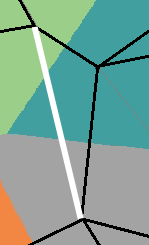
\includegraphics[width=0.3\linewidth]{blocking-example2}
	\caption{The white edge is an example of where the Distributed Greedy Voronoi Heuristic can fail to find an edge without peer management preventing this case.}
	\label{occ-ex}
\end{figure}


This is mitigated by our method of peer management described in subsection D and already present in Algorithm \ref{DGVH}.


\subsection{Fast Vornoi Classifier}
VHash never actually calculates the polytopes that describe a node's Voronoi region.
This is unnecessary and prohibitively expensive \cite{raynet}.
Rather VHash only ever assigns a given point to a Voronoi region.
It does this by calculating the distance from that point to all candidate nodes.
The point falls into a node's Voronoi region if it is the node to which it has the shortest distance.
Thus a node defines it's Voronoi region by keeping a list of the peers that bound it.

\subsection{Peer Management}
VHash maintains two peer lists: Short Peers and Long Peers.
This is motivated by mitigating the error induced by the Distributed Greedy Voronoi Heuristic and providing robustness during churn\footnote{The disruption caused to the overlay by the continuous joining, leaving, and failing of nodes.}.

Short Peers are the subset of the Delaunay Peers generated by the Distributed Greedy Voronoi Heuristic. 
The number of short peers has no upper bound and in contrived cases, such as a single node surrounded by other nodes forming a hypersphere, it can grow quite high. Previous work as found a useful lower bound on peers to be $3d + 1$\cite{raynet}
Using a lower bound on the length of the short peer list corrects for errors in the approximation processes by including peers that otherwise would not be. 
An approximation of the number of nodes in the network is sufficient to generate an accurate expected number of short peers.  
This expected number of short peers is used as the lower bound for the size of short peer list.
Should the number of short peers generated by the Distributed Greedy Voronoi Heuristic be less than the lower bound for that set's size, the nearest peers not already included in the short peer list are added to the short peer list until it is of sufficient size.
Short peers are analogous to the predecessors/successors in other DHTs.

Long Peers correspond to the two hop peers of the node.
When a node learns about potential neighbors, but are not included in the short peer list, they may be included in the long peer list.  
The long peer list has a maximum size of the base length of the short peer list squared.  
For example, if the short peer list has a minimum size of 8, the long peer list has a maximum size of 64 entries.  
Long peers are not actively probed during maintenance and the cost of managing them is minimal.
 
We discuss how nodes learn about short and long peers in the Gossiping subsection.


\subsection{Maintenance via Gossiping}
Each node in the network performs maintenance periodically by `gossiping' with a randomly chosen neighbor.
When two nodes gossip with each other, they exchange their short peer lists with each other.
The node combines the lists of short peers\footnote{Naturally, nodes remove themselves and repetitions from the candidates.} and uses the  Distributed Greedy Voronoi Heuristic to determine which of these candidates correspond to its neighbors along the Delaunay Triangulation.
The candidates determined not to be short peers become long peers.  
If resulting number of long peers exceeds the maximum size of the long peer list, a random subset of the maximum size is kept.

The formal algorithm for this process is described in \ref{gossip}.
This maintenance through gossip process is very similar to the gossip protocol used in \cite{raynet}.


\begin{algorithm}
\caption{Gossip Process}
\label{gossip}
\begin{algorithmic}[1]  % the number is how many 
	\STATE Node $n$ initiates the gossip.
	\STATE $neighbor \leftarrow$ random node from $n.short\_peers$
    \STATE $candidates \leftarrow n.short\_peers \cup neighbor.short\_peers$.
    \STATE $n$ and $neighbor$ each run Distributed Greedy Voronoi Heuristic using their own copy of $candidates$
\end{algorithmic} 
\end{algorithm}



\subsection{Handling Churn}
Churn is effects of the continuous joining and exiting of nodes in the overlay.
DHTs must have some mechanisms to handle this process to maintain fault tolerance and routing.

Joining the network is a straightforward process.  
A prospective node must be able to communicate with at least one patron member of the DHT.  
The prospective node is assigned a location using the method described in Section III and uses the patron it knows to find the node responsible for it's assigned location, which we call the parent.
The prospective node sets the parent node as the lone member of the short peers and immediately gossips with the parent.
Subsequent gossips will refine the peer lists of the nodes affected by the join.

There is no ``polite'' exit from the network. VHash assumes nodes will fail and the distinction between an intended failure and unintended failure is unnecessary.
Should a node wish to crease participating in the network, it need only to crease sending and receiving messages.
Suppose a node $f$ fails or leaves the network; we assume it does so abruptly and without warning.
When one of $f$'s neighbors attempts to contact $f$ for gossiping or routing, failure to communicate with $f$ will prompt the neighbor to remove $f$ from its peers.  
The node the selects a different neighbor to gossip with or recomputes the peer closest to the location it was looking for. 
Should a short peer fail, routing around its failure is trivial due to knowledge about the long peers.

\subsection{Routing}
The proper forwarding peer for routing a message extends from the voronoi regions of the short peers and long peers.
Rather than attempt to know the true voronoi region of those peers we approximate the voronoi regions of those peers as if there where no other nodes in the network.
The resulting voronoi regions describe both the subset of the network for which that peer is responsible and the subset of the network for which it is the most efficient forwarding node.
The routing node determines the voronoi region into which the message's destination falls.
If this is itself, it handles the message accordingly; otherwise the routing node forwards the message to the responsible node.
This process is equivalent to a pre-computed and cached efficient routing algorithm (Algorrihm \ref{lookup}).
Even if our approximation for the Voronoi region of a peer is incorrect due to incomplete knowledge of the network, our approximation describes the most efficient forwarding path of a message  destined for that space available.

\begin{algorithm}
\caption{Vhash Lookup}
\label{lookup}
\begin{algorithmic}[1] 
	\STATE $n$ is this node
	\STATE $m$ is a message addressed for $loc$
    \STATE $potential\_dests \leftarrow n \cup n.short\_peers$
    \STATE $c \leftarrow $ node in $ potential\_dests$ with shortest distance to $loc$
    \IF{$c$ == $n$}
    	\RETURN $n$
    \ELSE
        \RETURN c.lookup($loc$)
    \ENDIF
\end{algorithmic}
\end{algorithm}



\subsection{Algorithm Analysis}
The Distributed Greedy Voronoi Heuristic is very efficient in both terms of space and time.  Suppose a node is creating its short peer list from $k$ candidates.  The candidates must be sorted, which takes $O(k\cdot\lg(k))$ operations.  Then for each candidate, that the node must compute the midpoint between itself and the current candidate and then compare distances to that point between itself and all of the peers it has found so far.  This comes down to a cost of 

\[ k\cdot\lg(k) + k \text{ midpoint computations}  + k^{2} \text{ distance computations} \]


Since  $k$ is  bounded by $\Theta(\frac{\log N}{\log \log N} )$ \cite{bern1991expected} (the maximum number of peers stored neighbors allowed between two neighbors), we can translate the above to

\[O(\frac{\log^{2} N}{\log^{2} \log N} )\]

Because in the vast majority of cases, the number of peers is equal to the constant minimum table size, which gives $k=O(1)$ in the expected case, the lower bound and expected complexities  are $\Omega{}(1)$.

While previous work \cite{raynet} claims constant time approximation, the reality is that Raynet's leading constant is in the order of thousands as Monte-Carlo samples.  
While our algorithm has a greater asymptotic worst case cost, for all current realistic network sizes it will be more time efficent then raynet's approximation.



\section{Network Metric Embedding}
During previous research in applications of DHTs to parallel processing \cite{andrew-poster} we tested our network's behavior under churn.
We came to the unexpected conclusion that high levels of churn improved the performance of the system rather than being detrimental under the right circumstances.
The built-in mechanisms for managing responsibility in a DHT are very effective and efficient at handling servers changing locations in the network.
We found in this previous work that it was more effective to move the server to a location in the DHT where work or data was stored rather than attempt to remap data efficiently over the servers.
VHash is designed to leverage this discovery and allow a server's location in the network to provide meaningful information about the server and to allow servers to change location in the network to suit the networks needs.
In this paper we propose a method that peers can use to periodically change their location in the network such that routes taken on the resulting overlay network have lower latency than would otherwise possible in a DHT.\footnote{Is this better suited for Section I?}

We utilize a distributed graph embedding algorithm to find locations in the coordinate system for each node such that the latency between nodes can be accurately represented.
Once inter-node latency is effectively represented as distance in the coordinate space, routing for shortest distance across this space also routes along the shortest latency path on the overlay network.

For our simulations we measure latency in terms of hops on a large scale free graph (10,000 nodes) that acts as an underlying network.
We simulate a small fraction of these nodes to act as members of a DHT and simulate VHash's and Chord's distributions of latency for recursive lookups.
Each node in the VHash DHT preforms a periodic update step to it's location to accurately represent inter-node latency on the coordinate system.
We utilize a toroidal metric space for these experiments as generalization of Chord's ring topology.
Other research shows we have potential for even more effective results on a hyperbolic plane based coordinate system \cite{papadopoulos2010greedy}.

To preform the embedding we designed an algorithm based on force-directed graph drawing \cite{Spring} for servers to utilize and periodically update their locations to lower the latency with their peers.
The approximate distributed embedding algorithm utilizes VHash's maintenance and join behaviors.
This algorithm is described in Algorithm \ref{springalg}. Each node periodically measures the latencies to it's peers and generates a change in position that minimizes the error in distance to it's peers.
Once a node finds peers of low latency with it, these error approximations become small and the network configuration becomes stable.
If a node has high latency with it's current peers the high latency connection causes the nodes to repel each other and move to new peers.

\begin{algorithm}
\caption{Decentralized Peer-to-Peer Spring Model}
\label{springalg}
\begin{algorithmic}[1] 
	\STATE $n$ is a node at location $\overrightarrow{loc}$
    \STATE $total\_dist \leftarrow \sum distance(n,p),\forall p \in n.short\_peers$
    \STATE $total\_lat \leftarrow \sum latency(n,p),\forall p \in n.short\_peers$
    \STATE $unit\_lat \leftarrow total\_dist \div total\_lat$
    \FORALL{$p \in n.short\_peers$}
    	\STATE $ideal\_distance \leftarrow latency(n,p) \div unit\_lat$
        \STATE $error\_distance \leftarrow ideal\_distance - dist(n,P)$
        \STATE $\overrightarrow{loc} \leftarrow \overrightarrow{loc} + error\_distance \cdot \overrightarrow{Unit\_vector(n,p)} $
    \ENDFOR
\end{algorithmic}
\end{algorithm}
%Given node $N$, with random location $L_N$ and peers $P$
%Claculate the sum of $N$'s distances to all nodes in $P$, \%$total_distance$
%Calculate the sum of $N$'s latencies to all nodes in $P$, $total_latency$
%Unit latency per distance is approximately $total_distance$/$total_latency$



%While encoding latitude and logitude as locations and using distance across the earth's surface as the distance metric may provide an approximation of a minmum latency overlay topology, this method cannot be used in more general network sinarios and may not describe the actual lowest latency path.



\section{Simulations}
We implemented two simulations to prove that VHash acts as as a stable DHT and is able to minimize the latency on lookup time.
Our first simulation was of successful lookup rates (hitrate) over time as a VHash overlay converged on the proper topology from a random graph.  
This simulated a large network bootstrapping itself from a series of essentially random connections and into an ordered DHT.
  
Our other simulation compared the distributions of latency in both the VHash and Chord DHTs to examine VHash's capability to minimize latency. 
We wanted to demonstrate the benefits to latency that followed from optimizing VHash's overlay topology for minimum latency according to our spring model (Algorithm \ref{springalg}).

% Routing convergence tests
\subsection{Convergence Simulation}
This simulation demonstrates that the VHash protocol converges to a stable overlay from an chaotic starting topology after a sufficient number of gossip cycles.  
We do this by showing that rate of successful lookups converges to 1.0.
We compare these results to RayNet \cite{raynet}, which proposed that a random $k$-connected graph would be a good, challenging starting configuration for demonstrating convergence of a DHT to a stable network topology.

During the first two cycles of the simulation, each node bootstraps its short peer list by appending 10 randomly selected nodes.
In all the cycles, the nodes perform a gossip with a random node from their short peers to recompute both their peer lists.
We then calculate the hitrate of successful lookups by simulating 2000 lookups from random nodes to random locations, as described in Algorithm \ref{routesim}.

Our experimental variables for this simulation were the number of nodes in VHash overlay and the number of dimensions.  
We tested network sizes of 500, 1000, 2000, 5000, and 10000 nodes each in 2, 3, 4, and 5 dimensions.
The hitrate at each cycle is $\frac{hits}{2000}$, where hits are the number of successful lookups.

 


\begin{algorithm}
\caption{Routing Simulation Sample}
\label{routesim}
\begin{algorithmic}[1]  % the number is how many 
	\STATE $start \leftarrow$ random node
	\STATE $dest \leftarrow$ random set of coordinates
    \STATE $ans \leftarrow$ node closest to $dest$
    \IF{$ans == start.lookup(dest)$}
    	\STATE increment $hits$
    \ENDIF
\end{algorithmic} 
\end{algorithm}


%In order to show that leaving the size of the short peer list unbounded is not detrimental to the memory costs of nodes, we also kept track of the size of the short peer list at each cycle. 

%\subsection{Convergence Simulation Results}
Our results are shown in Figures \ref{conv2} \ref{conv3} \ref{conv4}.
Our graphs show that VHash's overlay quickly constructs itself from a random configuration and that our hitrate approached 90\% by cycle 20, regardless of dimension.
VHash consistently converged to a hitrate of 1.0 by cycle 30. 
In comparison, Raynet's routing converged to a perfect hitrate at around cycle 30 to 35 \cite{raynet} 
As the network size and number of dimensions each increase, convergence slows, but not to a significant degree.
 


\begin{figure}
	\centering
	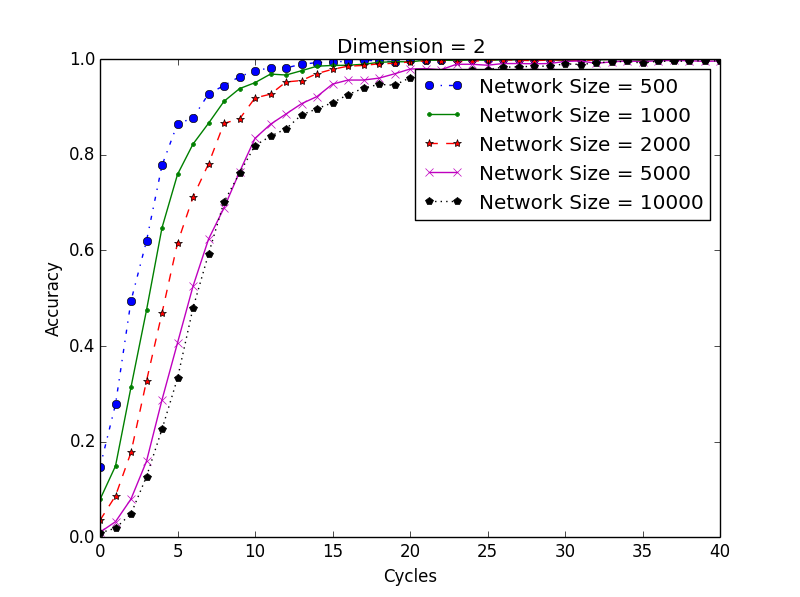
\includegraphics[width=\linewidth]{conv_d2}
	\caption{}
	\label{conv2}
\end{figure}


\begin{figure}
	\centering
	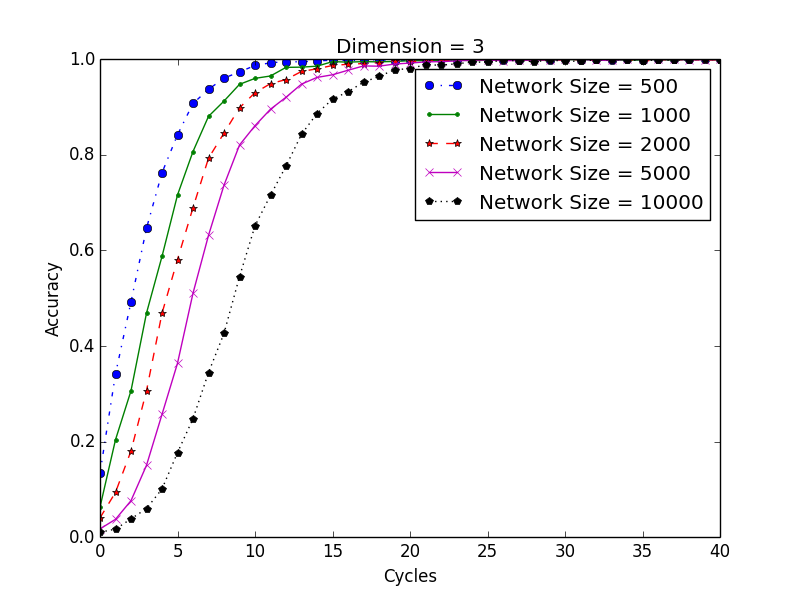
\includegraphics[width=\linewidth]{conv_d3}
	\caption{}
	\label{conv3}
\end{figure}

\begin{figure}
	\centering
	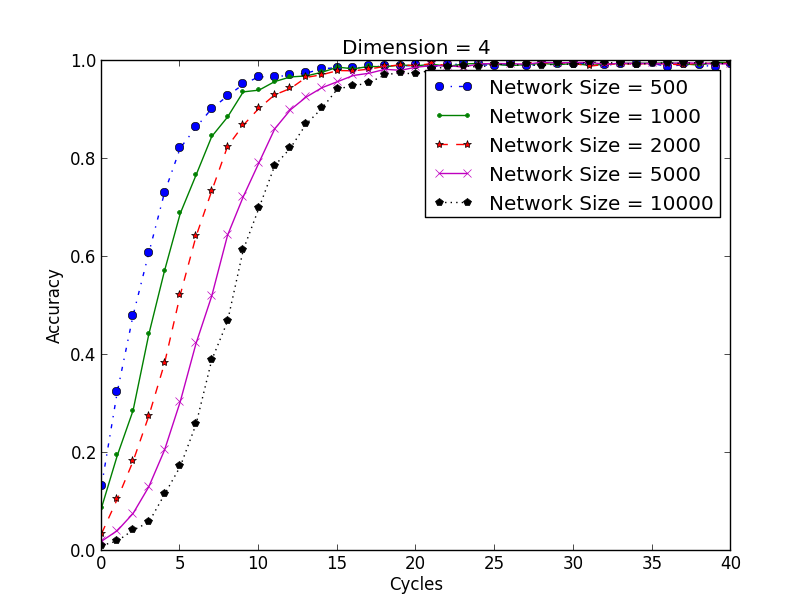
\includegraphics[width=\linewidth]{conv_d4}
	\caption{}
	\label{conv4}
\end{figure}






%\begin{table}
%\centering
%\begin{tabular}{|r|r|r|r|}
%\hline
%Network Size & Dimensions & avg degree & max degree\\ \hline
%500   & 2 & 7.004 & 8 \\ \hline
%1000  & 2 & 7.001 & 8 \\ \hline
%2000  & 2 & 7.0015 & 8 \\ \hline
%5000  & 2 & 7.0364 & 66 \\ \hline
%10000 & 2 & 8.0151 & 81\\ \hline  % the heck?
%500   & 3 & 10.364 & 16 \\ \hline
%1000  & 3 & 10.321 & 15 \\ \hline
%2000  & 3 & 10.272 & 16 \\ \hline
%5000  & 3 & 10.3264 & 18 \\ \hline
%10000 & 3 & 9.1233 & 19 \\ \hline
%500   & 4 & x & x \\ \hline
%1000  & 4 & x & x \\ \hline
%2000  & 4 & x & x \\ \hline
%5000  & 4 & x & x \\ \hline
%10000 & 4 & x & x \\ \hline
%500   & 5 & x & x \\ \hline
%1000  & 5 & x & x \\ \hline
%2000  & 5 & x & x \\ \hline
%5000  & 5 & x & x \\ \hline
%10000 & 5 & x & x \\ \hline
%\end{tabular}
%\caption{Information about the size short peer lists, denoted degree here, at the last cycle of the convergence simulation.  For each pair of network size and dimension, we report the average degree in the network, as well as the largest.}
%\label{tab:convtable}
%\end{table}






% Hop distance test
\subsection{Latency Distribution Test}
The goal of our second set of experiments is to demonstrate VHash's ability to optimize a selected network metric: latency in this case.  
We compared VHash's performance to that of a more traditional DHT, Chord \cite{chord}.
Chord is a well established DHT with an $O(log(n))$ sized routing table and $O(log(n))$ lookup time measured in overlay hops.  
Rather than examine the number of hops on the overlay network as our primary metric as done most other analyses of lookup time \cite{chord} \cite{pastry} \cite{raynet}  \cite{kademlia} \cite{voronet}, we are concerned with the actual latency lookups experience traveling through the \emph{underlay} network, the network the overlay is built upon.

For this experiment we constructed a 10000 node random scale free network (which has an approximate diameter of 3 hops) to act as an underlay \cite{cohen2000resilience} \cite{pastor2001epidemic} \cite{hagberg2004}.
We used a scale-free network as the underlay as it is a simplified model of the Internet's topology \cite{cohen2000resilience} \cite{pastor2001epidemic}.
From this underlay, we chose a random subset to be members of the overlay network.
We then measured the distance in underlay hops between 10000 random source-destination nodes from the overlay. 
VHash generates an embedding of the latency graph utilizing the distributed spring model algorithm described in Algorithm \ref{springalg}, with the latency function is defined as the number of underlay hops between it and its peers.
%we should elaborate more as to why underlay hops are a good measure of latency
Overlay hops are used in most DHT papers as the primary measure of latency under the rationale that as the number of nodes increases towards maximum network capacity, the majority of nodes will have average latency with the majority of other nodes because the nodes will be more uniformly distributed.
This rationale is only valid where it's assumption of massive and diverse networks is held.
For most realistic network sizes and structures, there is dramatic room for latency reduction in DHTs.

%pictures here


\begin{figure}
	\centering
	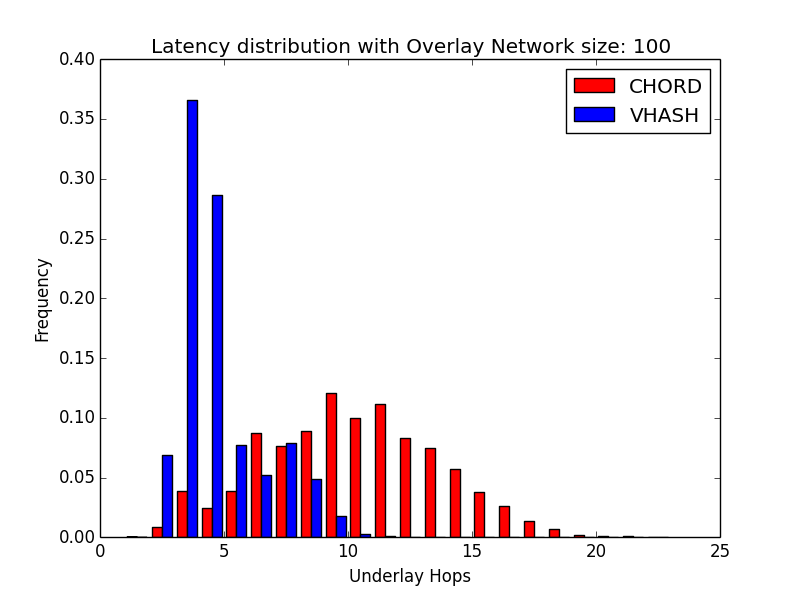
\includegraphics[width=\linewidth]{hist_100}
	\label{hist100}
\end{figure}

\begin{figure}
	\centering
	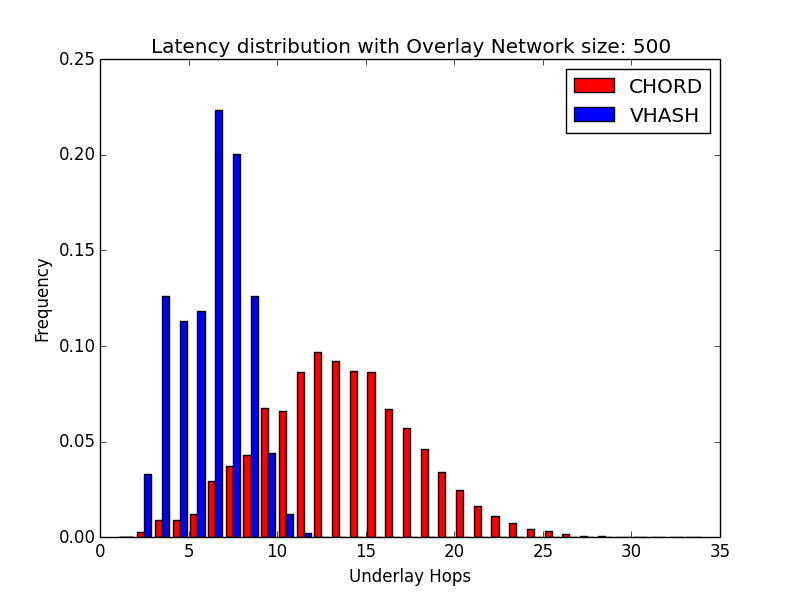
\includegraphics[width=\linewidth]{hist_500}
	\label{hist500}
\end{figure}

\begin{figure}
	\centering
	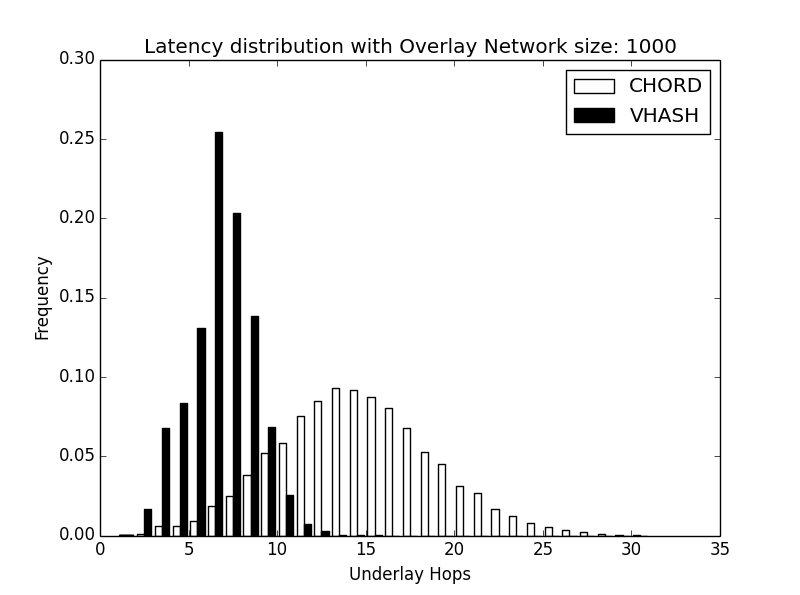
\includegraphics[width=\linewidth]{hist_1000}
	\label{hist1000}
\end{figure}



\begin{figure}
	\centering
	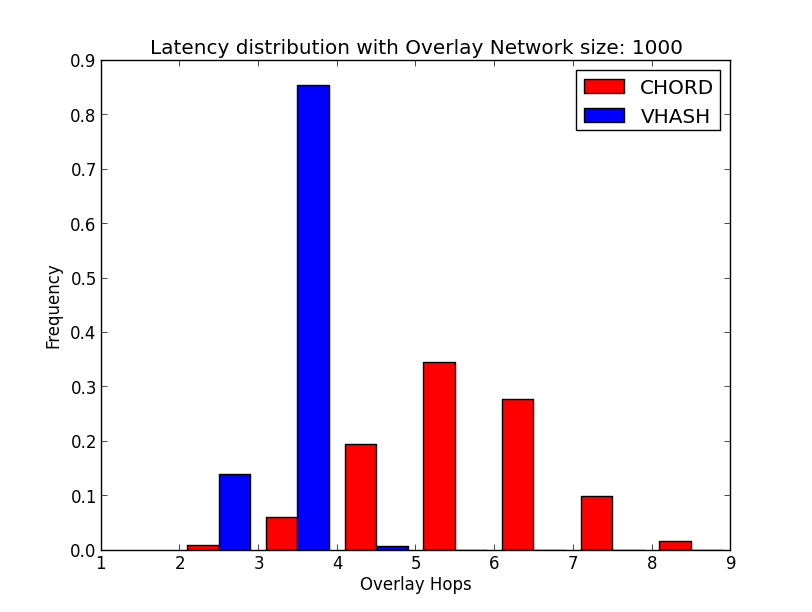
\includegraphics[width=\linewidth]{hist_overlay_4d}
	\caption{Comparison of Chord and VHash in terms of overlay hops.  Each overlay has 1000 nodes.}
	\label{hist1000}
\end{figure}


VHash performs better in both minimum underlay and overlay hops


\subsection{Conclusions}
In general, in similar circumstances, VHash converges faster than RayNet.
Convergence rate varies with network size and number of dimensions of the VHash space.
Utilizing the current latency-embedding technique VHash is useful for building DHT networks of reasonable size.

\section{Related Work}
%check table size consistancy 
While there has been previous work on applying Voronoi regions to DHTs and P2P applications, we have found no prior work on how to perform embedding of an inter-node latency graph.   

Backhaus et. al's  VAST \cite{Backhaus:2007:VAS:1326257.1326266} is a Voronoi-based P2P protocol designed for handling event messages in a massively multiplayer online videogame.  
Each node finds its neighbors by constructing a Voronoi diagram using Fortune's sweepline algorithm \cite{fortune1987sweepline}.  
VAST demonstrated that Voronoi diagrams could be used as the backbone  large-scale, although their work focused specifically on using 2-dimensional Voronoi diagrams.  
VHash approximates the Voronoi region rather than solving it, as higher dimension Voronoi regions are computationally expensive to solve.
In addition, VHash is designed to exploit network metrics.

The two DHT protocols developed by Beumont et al., VoroNet \cite{voronet} and RayNet \cite{raynet} are the closest comparisons to VHash.
VoroNet is based off Kleinberg's small world model \cite{kleinberg2000navigation} and achieves polylogarithmic lookup time.  
Each node in Voronet solves its Voronoi region to determine its neighbors and also maintains a link to a randomly chosen distant node.
Voronet focused specifically on the two-dimensional Vornoi computations and the techniques used would be too expensive in higher dimensions and were not resilient to churn  \cite{raynet}.

RayNet \cite{raynet} was based on the work done on Voronet and is by far the most similar to VHash.  
Like VHash, RayNet does not solve for Voronoi regions, as that is prohibitively expensive.  
Unlike VHash, RayNet uses a Monte-Carlo method to approximate the volume of a node's Voronoi region.  
While effective and estimating the Voronoi region,  the volume-based Monte-Carlo approximation is expensive and requires multiple samples. 
RayNet does mention the idea of mapping attributes to each axis, but how this can be exploited is left as future work.



 

\section{Conlusions and or Future Work}
\begin{itemize}
\item Explore applications of metric spaces.
\item Explore file management and backup method.
\item Explore caching and replication strategies.
%\item Find better table sizes?  We kinda just chose ours on an ad-hoc basis
\end{itemize}



\bibliographystyle{ieeetr}
\bibliography{P3DNS}
\end{document}
